\section{Versuchsaufbau/-durchführung}
Zur experimentellen Untersuchung des Photoeffektes wird der Aufbau nach Abbildung \ref{fig: aufbau} verwendet. Eine
genauere Darstellung der Photozelle befindet sich in Abbildung \ref{fig: photozelle}. Hierbei handelt es sich um einen
evakuierten Glaskolben, der im Inneren zwei Elektroden einschließt. Die Kathode stellt eine aufgedampfte
Metallschicht dar, die mit Licht bestrahlt werden kann. Die Anode ist als Drahtring realisiert, der parallel
zur Kathode angebracht ist. Werden nun Elektronen aus der Kathode ausgelöst, ist zwischen den beiden Elektroden
mit einem Nanoamperemeter ein Strom messbar. \\ %Nanoampermeter
Um die kinetische Energie der ausgelösten Elektronen zu untersuchen wird die Gegenfeldmethode angewandt. Ein Schaltplan
dieser Anordnung ist in Abbildung \ref{fig: schaltplan} dargestellt. Die Elektronen müssen gegen ein elektrisches Feld anlaufen.
Wird die Gegenspannung $U$ erhöht, so sollte ab einer Grenzspannung der Photostrom zum erliegen kommen. Es gilt dann
für die kinetische Energie der Elektronen
\begin{align}
  \label{eq:regress}
\begin{aligned}
  e\ua{0} U\ua{G} &= \frac{1}{2}m\ua{e}v^2 \\
  \Rightarrow h\nu &= e\ua{0}U\ua{G} + A\ua{k}.
\end{aligned}
\end{align}
Dieser Zusammenhang ermöglicht eine Bestimmung der Größe $\frac{h}{e\ua{0}}$. Es ist zu beachten, dass
die kinetische Energie der Elektronen einer Fermi-Dirac-Verteilung genügen. Die Elektronen
besitzen daher unterschiedliche Geschwindigkeiten und der Photostrom fällt nicht abrupt sondern
stetig auf null ab. Zwischen dem Photostrom $I\ua{ph}$ und der Gegenspannung $U\ua{G}$ besteht im betrachteten Bereich ein quadratischer Zusammenhang
\begin{equation}
  I\ua{ph} \propto U^2.
\end{equation}
Als Lichtquelle wird im Versuch eine Quecksilberlampe verwendet, deren Licht mit einer Linsenanordnung gebündelt
und einem Geradsichtprisma in seine Spektrallinien aufgespalten wird. Mittels eines Schwenkarms kann das Schutzgehäuse
so eingestellt werden, dass nur die zu untersuchende Lichtfarbe in die Photozelle fällt. Die Abhängigkeit zwischen
Photostrom und Gegenspannung wird für gelbes, grünes, blau-grünes, violettes und ultraviolettes Licht untersucht. Dazu
werden jeweils etwa zehn Messpunkte aufgezeichnet. Für gelbes Licht wird darüber hinaus die Abhängigkeit des Photostromes
von der Spannung zwischen Anode und Kathode untersucht. Dabei wird die Spannung in dem Aufbau nach Abbildung \ref{fig: aufbau}
sowohl bremsend als auch beschleunigend gerichtet angelegt.
\begin{figure}
  \centering
  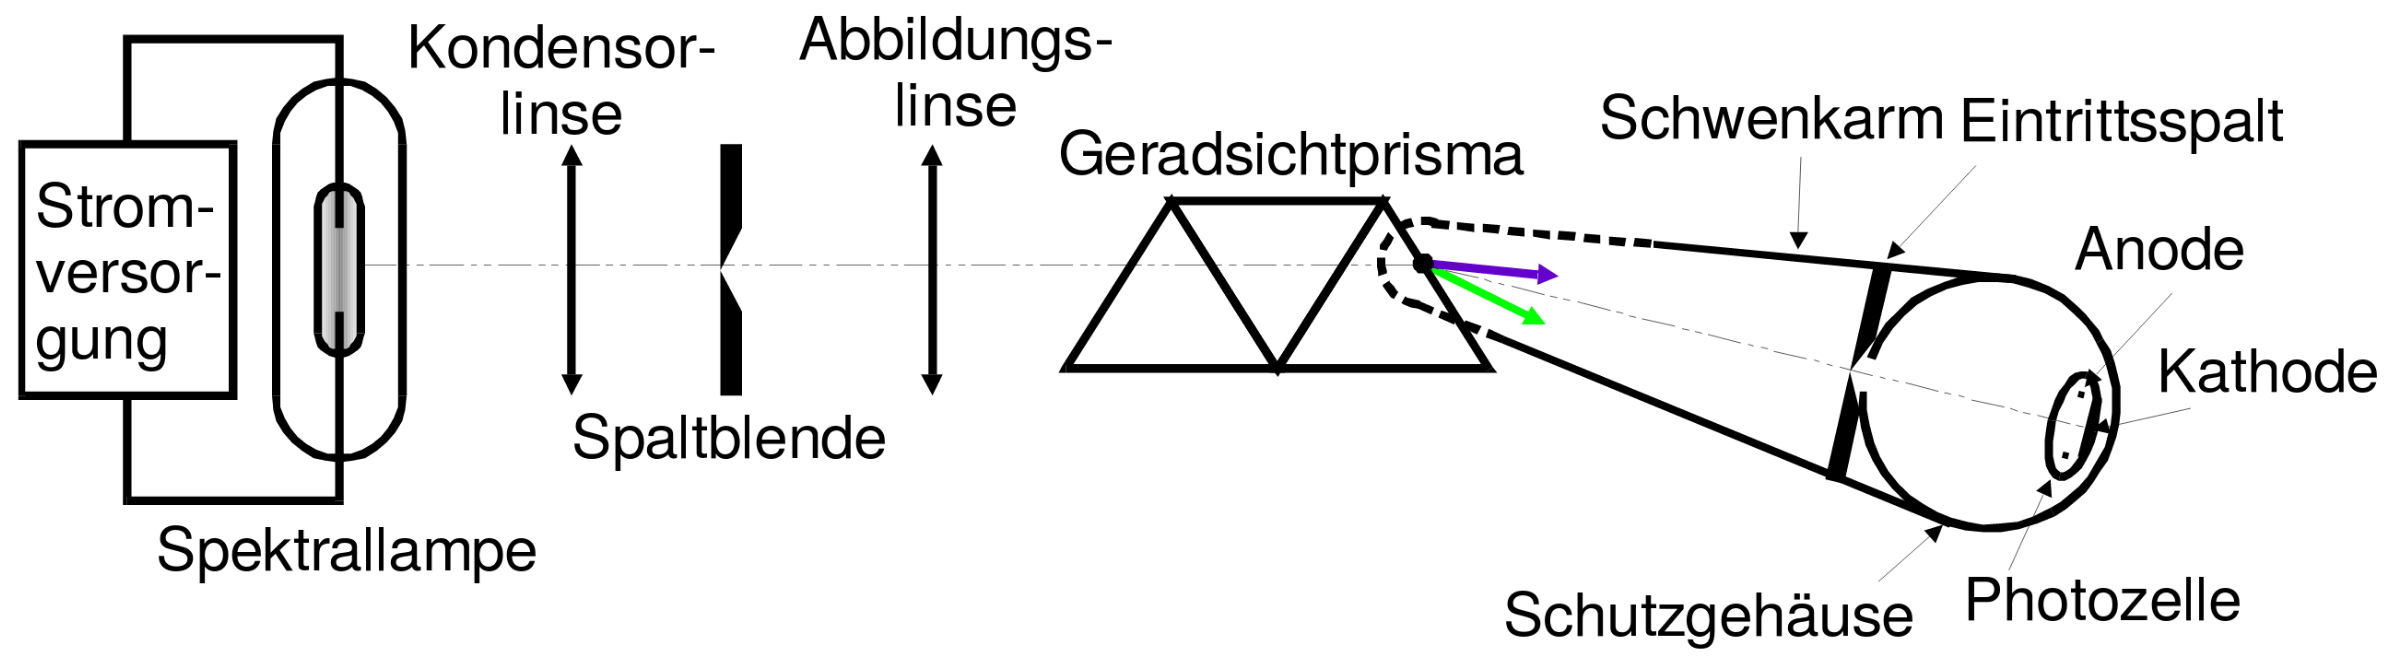
\includegraphics[width = 0.7\textwidth]{pics/aufbau.png}
  \caption{Versuchsaufbau zur Untersuchung des Photoelektrischen Effekts \cite{anleitung500}.}
  \label{fig: aufbau}
\end{figure}
\begin{figure}
  \centering
  \begin{subfigure}{0.48\textwidth}
    \centering
    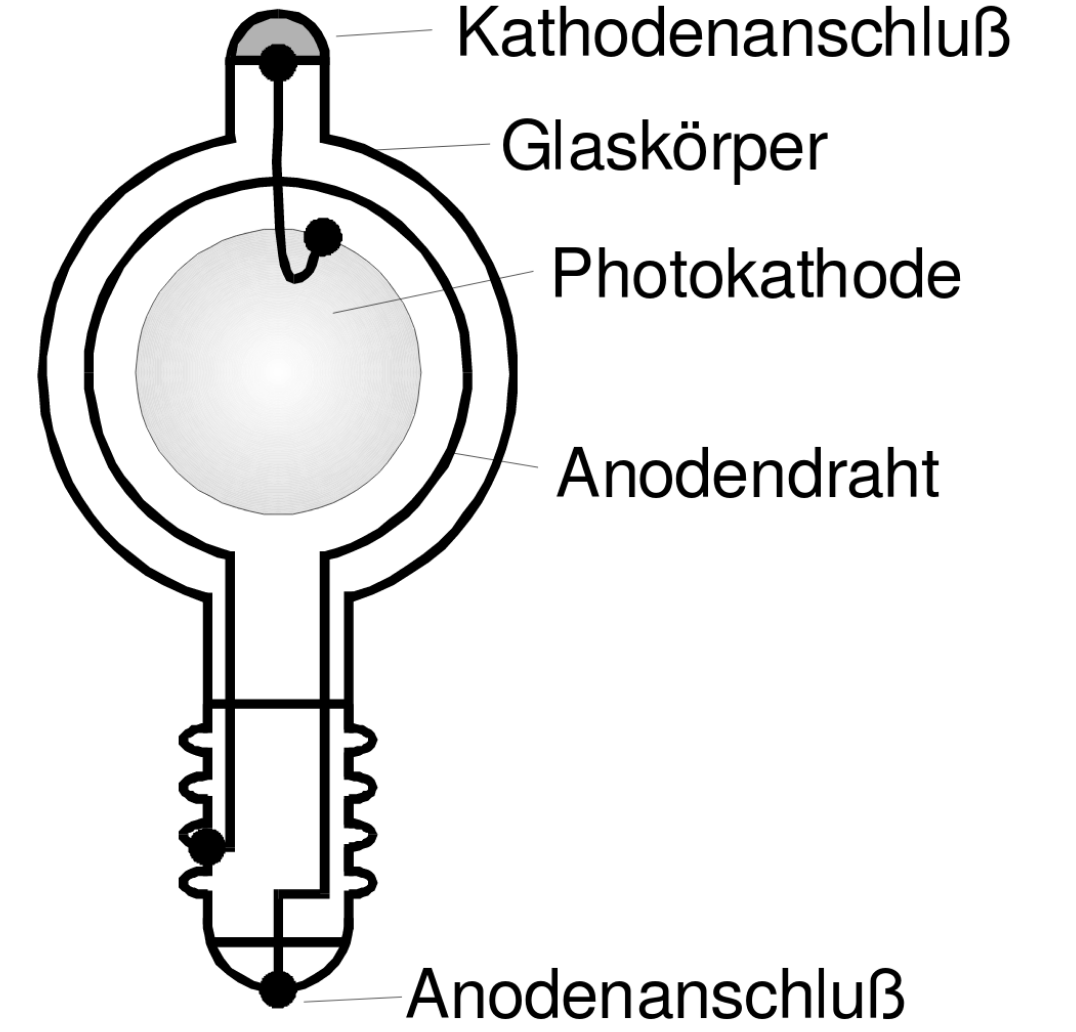
\includegraphics[width = 0.5\textwidth]{pics/photozelle.png}
    \caption{Photozelle \cite{anleitung500}.}
    \label{fig: photozelle}
  \end{subfigure}
  \begin{subfigure}{0.48\textwidth}
    \centering
    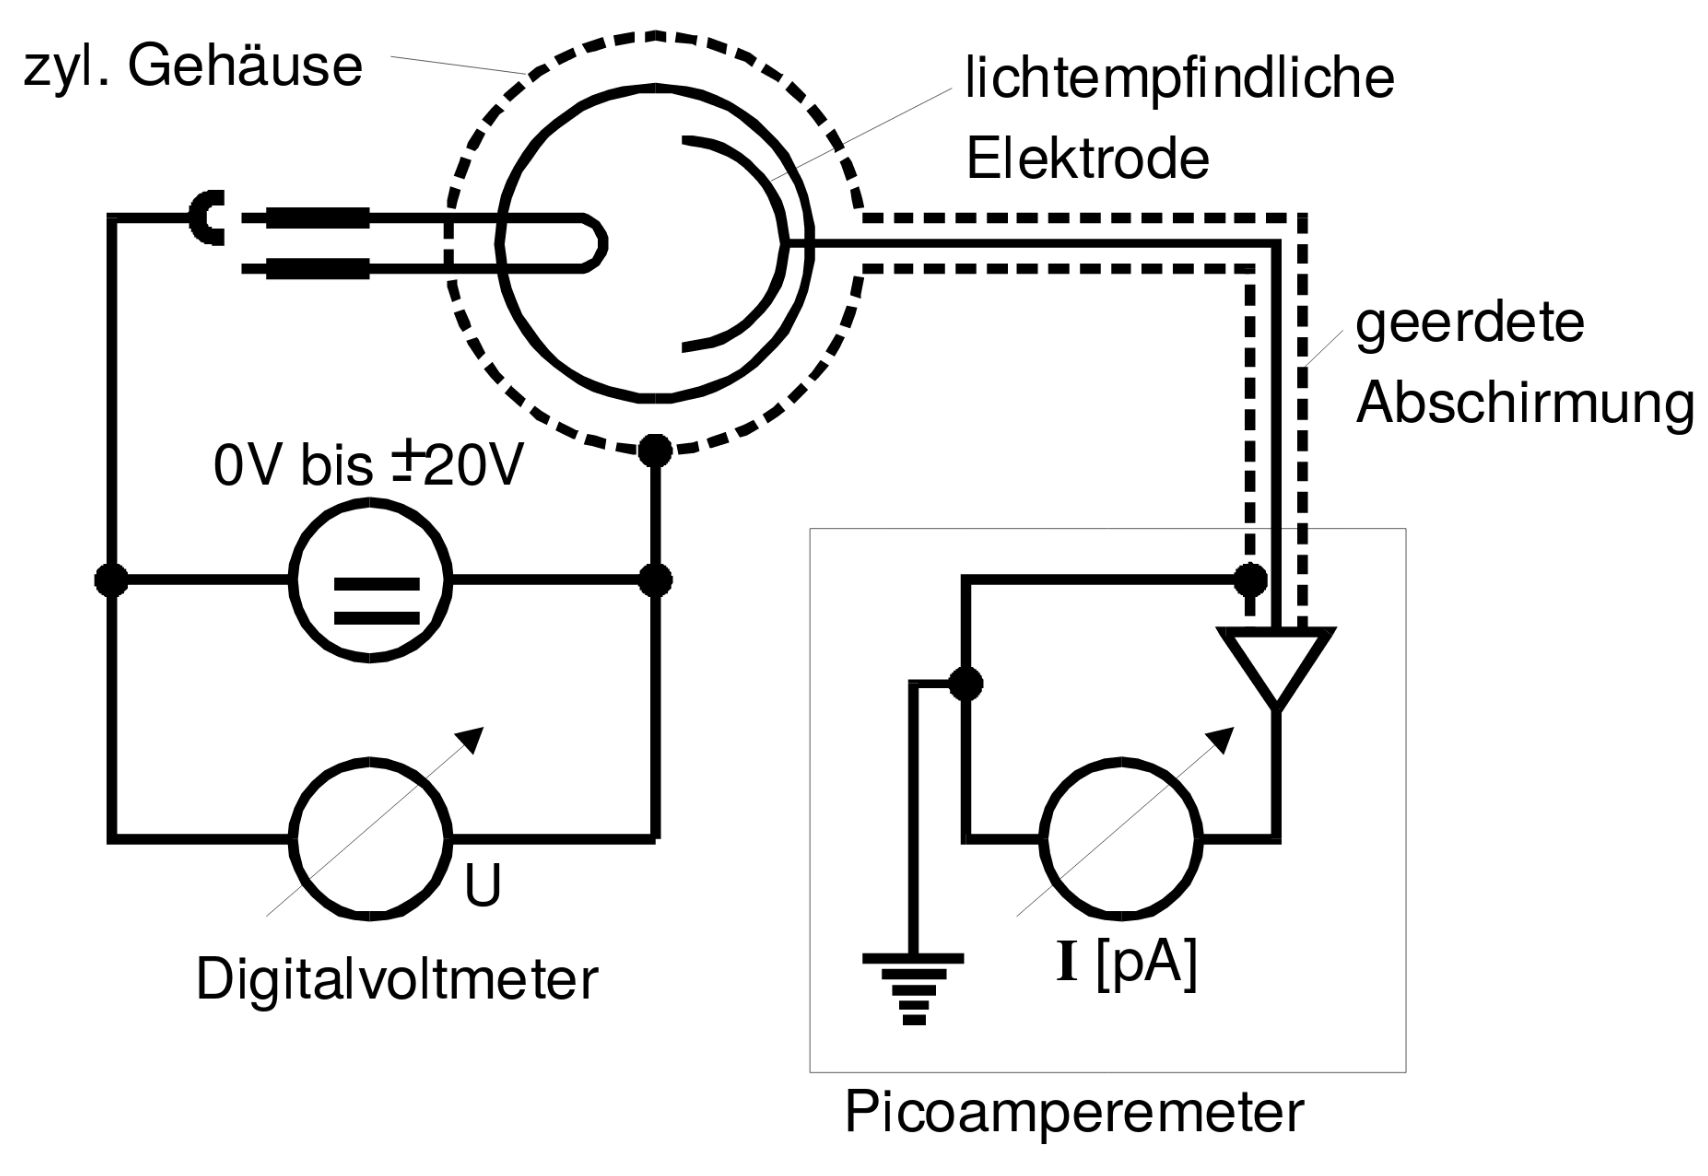
\includegraphics[width = 0.7\textwidth]{pics/schaltplan.png}
    \caption{Schaltung für die Gegenfeldmethode \cite{anleitung500}.}
    \label{fig: schaltplan}
  \end{subfigure}
  \caption{Schematische Darstellungen der Photozelle und des Aufbaus zur Gegenfeldmethode.}
\end{figure}
